%%% LaTeX Template
%%% This template is made for project reports
%%%	You may adjust it to your own needs/purposes
%%%
%%% Copyright: http://www.howtotex.com/
%%% Date: March 2011

%%% Preamble
\documentclass[10pt]{report}	% Article class of KOMA-script with 11pt font and a4 format

\usepackage{color}
\usepackage{framed}
\usepackage{textcomp}
\usepackage{listings}
\usepackage{hyperref}
\usepackage[page]{appendix}
\usepackage{graphicx}
\usepackage{verbatim}
\usepackage{amsmath}
\usepackage{xspace}
%\usepackage{minitoc}
\usepackage{mtcoff}
\usepackage[tt]{titlepic}
\usepackage{array}

\usepackage{sstmacro}

\usepackage[textwidth=6.5in]{geometry}

\definecolor{shadecolor}{rgb}{1,0.8,0.3}
\definecolor{dkgreen}{rgb}{0,0.6,0}
\definecolor{purple}{rgb}{1,0,1}

\newcommand{\todo}[1] {\textcolor{red}{-[#1]-}}


\newcommand{\mytilde}{{\raise.17ex\hbox{$\scriptstyle\sim$}}}

\newcommand{\sstmacro}{{SST/\raise.35ex\hbox{macro}}\xspace}
\newcommand{\sprockit}{{SProCKit}\xspace}
\newcommand{\eg}{\textit{e.g.}}

\newcommand{\class}[1]{\textcolor{blue}{#1}}

\newcommand{\func}[1]{\textcolor{purple}{#1}}

\newcommand{\folder}[1]{\textcolor{dkgreen}{#1}}

\newcommand{\aside}[1]{\begin{framed} #1 \end{framed}}

\newcommand{\guikey}[1]{\emph{#1}}

\newcommand{\inlinefile}[1]{{\lstset{basicstyle=\ttfamily,keywordstyle={}}\lstinline$#1$}}

\newcommand{\inlinecode}[1]{{\lstset{basicstyle=\ttfamily,keywordstyle={},showstringspaces=false}\lstinline$#1$}}
\newcommand{\inlineshell}[1]{{\lstset{basicstyle=\ttfamily,keywordstyle={},showstringspaces=false}\lstinline$#1$}}

\title{SST/macro 6.1: Developer's Reference}

\author{Sandia National Labs \\ Livermore, CA}

\titlepic{
\includegraphics[width=0.3\textwidth]{figures/sstlogo.png}}

\setlength{\parindent}{0cm} % Default is 15pt.
\setlength{\parskip}{2mm plus1mm minus1mm}

\begin{document}

\maketitle 

\tableofcontents

% !TEX root = developer.tex

\chapter{Introduction}\label{chapter:intro}

\section{Use of C++/Boost}\label{sec:boost}
SST/macro (Structural Simulation Toolkit for Macroscale) is a discrete event simulator designed for macroscale (system-level) experiments in HPC. 
SST/macro is an object-oriented C++ code that makes heavy use of dynamic types and polymorphism.
While a great deal of template machinery exists under the hood, nearly all users and even most developers will never actually need to interact with any C++ templates.
Most template wizardry is hidden in easy-to-use macros.
While C++ allows a great deal of flexibility in syntax and code structure, we are striving towards a unified coding style.

\section{Polymorphism and Modularity}\label{sec:polymorphism}
The simulation progresses with different modules (classes) exchanging messages.
In general, when module 1 sendings a message to module 2, module 1 only sees an abstract interface for module 2.
The polymorphic type of module 2 can vary freely to employ different physics or congestions models without affecting the implementation of module 1. 
Polymorphism, while greatly simplifying modularity and interchangeability, does have some consequences.
The ``workhorse'' of SST/macro is the base \inlinecode{event} and \inlinecode{message} classes.
To increase polymorphism and flexibility, every SST/macro module that receives messages does so via the generic function

\begin{CppCode}
void
handle(event* ev){
...
}
\end{CppCode}
The prototype therefore accepts \emph{any} event type. The class \inlinecode{message} is a special type of event that refers specifically to a message (e.g. MPI message) carrying a data payload.
Misusing types in SST/macro is \emph{not} a compile-time error.
The onus of correct event types falls on runtime assertions.
All event types may not be valid for a given module.
A module for the memory subsystem should throw an error if the developer accidentally passes it a event intended for the OS or the NIC.
Efforts are being made to convert runtime errors into compile-time errors.
In many cases, though, this cannot be avoided.
The other consequence is that a lot of dynamic casts appear in the code.
An abstract \inlinecode{event} type is received, but must be converted to the specific message type desired.
NOTE: While \emph{some} dynamic casts are sometimes very expensive in C++ (and are implementation-dependent),
most SST/macro dynamic casts are simple equality tests involving virtual table pointers.

While, SST/macro strives to be as modular as possible, allowing arbitrary memory, NIC, interconnect components,
in many cases certain physical models are simply not compatible.
For example, using a fluid flow model for memory reads cannot be easily combined with a packet-based model for the network.
Again, pairing incompatible modules is not a compile-time error.
Only when the types are fully defined at runtime can an incompatibility error be detected.
Again, efforts are being made to convert as many type-usage problems into compiler errors.
We prefer simulation flexibility to compiler strictness, though. 

\section{Most Important Style and Coding Rules}\label{sec:stylerules}
Here is a selection of C++ rules we have tended to follow.  
Detailed more below, example scripts are included to reformat the code style however you may prefer for local editing.
However, if committing changes to the repository, only use the default formatting in the example scripts.
\begin{itemize}
\item snake\_case is used for variable and class names.
\item We use ``one true brace`` style (OTBS) for source files. 
\item In header files, all functions are inline style with attached brackets.
\item To keep code compact horizontally, indent is set to two spaces. Namespaces are not indented.
\item Generally, all if-else and for-loops have brackets even if a single line.
\item Accessor functions are not prefixed, i.e. a function would be called \inlinecode{name()} not \inlinecode{get_name()}, except
where conflicts require a prefix. Functions for modifying variables are prefixed with \inlinecode{set_},
\item We use .h and .cc instead of .hpp and .cpp
\item As much implementation as possible should go in .cc files.
	Header files can end up in long dependency lists in the make system.  
	Small changes to header files can result in long recompiles.
	If the function is more than a basic set/get, put it into a .cc file.
\item Header files with many classes are discouraged.  When reasonable, one class per header file/source file is preferred.
	 Many short files are better than a few really long ones.
\item Document, document, document.  If it isn't obvious what a function does, add doxygen-compatible documentation.
	Examples are better than abstract wording.
\item Use STL and Boost containers for data structures.  Do not worry about performance until much later.
	Premature optimization is the root of all evil. If determined that an optimized data structure is needed,
	please do that after the entire class is complete and debugged.
\item Forward declarations.  There are a lot of interrelated classes, often creating circular dependencies. In addition, you can add up with an explosion of include files, often involving classes that are never used in a given \inlineshell{.cc} file.  For cleanliness of compilation, you will find many \inlineshell{*_fwd.h} files throughout the code. If you need a forward declaration, we encourage including this header file rather than ad hoc forward declarations throughout the code.
\end{itemize}

\section{Code Style Reformatting}\label{sec:styleReformat}
Since we respect the sensitivity of code-style wars, we include scripts that demonstrate basic usage of the C++ code formatting tool \emph{astyle}.
This can be downloaded from {http://astyle.sourceforge.net}. 
A python script called \inlineshell{fix_style} is included in the top-level bin directory.
It recursively reformats all files in a given directory and its subdirectories.

\section{Memory Allocation}\label{sec:memalloc}
To improve performance, custom memory allocation strategies can be employed in C++.
At present, a global custom \inlinecode{operator new} can be optionally activated which is optimized for large pages and memory pools.
At present, no class-specific implementation of \inlinecode{operator new} is used.
However, we may soon implement custom allocation techniques to improve things like cache/TLB efficiency.
This is the only major change expected to SST/macro that would affect externally developed modules - and even here the expected modifications would be quite small.
Because custom allocation schemes may be used, all externally developed code should use \inlinecode{operator new}, rather than \emph{not}  \inlinecode{malloc} or \inlinecode{mmap}, unless allocating very large arrays.


% !TEX root = developer.tex

\chapter{SProCKit}\label{chapter:sprockit}
\sstmacro is largely built on the Sandia Productivity C++ Toolkit (\sprockit),
which is included in the \sstmacro distribution.
Projects developed within the simulator using \sprockit can easily 
move to running the application on real machines while still using the \sprockit infrastructure.
One of the major contributions is reference counted pointer types.
The parameter files and input deck are also part of \sprockit.

\section{Debug}\label{sec:debug}
The goal of the \sprockit debug framework is to be both lightweight and flexible.
The basic problem encountered in \sstmacro development early on was the desire to have very fine-grained control over when and where something prints.
Previously declared debug flags are passed through the \inlinecode{debug_printf} macro.

\begin{CppCode}
debug_printf(sprockit::dbg::mpi,
  "I am MPI rank %d of %d",
  rank, nproc);
\end{CppCode}

The macro checks if the given debug flag is active. 
If so, it executes a \inlinecode{printf} with the given string and arguments.
Debug flags are turned on/off via static calls to

\begin{CppCode}
sprockit::debug::turn_on(sprockit::dbg::mpi);
\end{CppCode}

\sstmacro automatically turns on the appropriate debug flags based on the \inlineshell{-d} command line flag
or the \inlineshell{debug = } parameter in the input file.

Multiple debug flags can be specified via OR statements to activate a print statement through multiple different flags.

\begin{CppCode}
using namespace sprockit;
debug_printf(dbg::mpi | dbg::job_launch,
  "I am MPI rank %d of %d",
  rank, nproc);
\end{CppCode}

Now the print statement is active if either MPI or job launching is going to be debugged.

In \inlineshell{sprockit/debug.h} a set of macros are defined to facilitate the declaration.
To create new debug flags, there are two macros.
The first, \inlinecode{DeclareDebugSlot}, generally goes in the header file to make the flag visible to all files.
The second, \inlinecode{RegisterDebugSlot}, goes in a source file and creates the symbols and linkage for the flag.

\begin{CppCode}
launch.h:
DeclareDebugSlot(job_launch);

launch.cc
RegisterDebugSlot(job_launch);
\end{CppCode}

\section{Serialization}\label{sec:serialize}
Internally, \sstmacro makes heavy use of object serialization/deserialization in order to run in parallel with MPI.
To create a serialization archive, the code is illustrated below. Suppose we have a set of variables

\begin{CppCode}
struct point {
 int x;
 int y;
}
point pt;
pt.x = 0;
pt.y = 2;
int niter = 5;
std::string str = "hello";
\end{CppCode}

We can serialize them to a buffer

\begin{CppCode}
sstmac::serializer ser;
ser.set_mode(sstmac::serializer::PACK);
ser.init(new char[512]);
ser & pt;
ser & niter;
ser & str;
\end{CppCode}
In the current implementation, the buffer must be explicitly given.

To reverse the process for a buffer received over MPI, the code would be

\begin{CppCode}
char* buf = new char[512];
MPI_Recv(buf, ...)
sstmac::serializer;
ser.set_mode(sstmac::serializer::UNPACK);
ser.init(buf);
ser & pt;
ser & niter;
ser & str;
\end{CppCode}

Thus the code for serializing is exactly the same as deserializing. The only change is the mode of the serializer is toggled.
The above code assumes a known buffer size (or buffer of sufficient size).
To serialize unknown sizes, the serializer can also compute the total size first.

\begin{CppCode}
sstmac::serializer ser;
ser.reset();
ser.set_mode(sstmac::serializer::SIZER);
ser & pt;
ser & niter;
ser & str;
int size = ser.sizer.size(); //would be 17 for example above
char* buf = new char[size];
...
\end{CppCode}
The known size can now be used safely in serialization.

The above code only applies to plain-old dataypes and strings.
The serializer also automatically handles STL containers
through the \inlinecode{&} syntax.
To serialize custom objects, a C++ class must implement the serializable interface.

\begin{CppCode}
namespace my_ns {
class MyObject : 
  public sstmac::serializable
{
 ImplementSerializable(my_object)
 ...
 void serialize_order(sstmac::serializer& ser);
 ...
};
}
\end{CppCode}
The serialization interface requires inheritance from \inlinecode{serializable}.
This inheritance forces the object to define a \inlinecode{serialize_order} function.
The macro \inlinecode{ImplementSerializable} inside the class creates a set of necessary functions.
This is essentially a more efficient RTTI, mapping unique integers to a polymorphic type.
The forced inheritance allows more safety checks to ensure types are being set up and used correctly.
All that remains now is defining the \inlinecode{serialize_order} in the source file:

\begin{CppCode}
void MyObject::serialize_order(sstmac::serializer& ser)
{
  ser & my_int_;
  set << my_double_;
  ...
}
\end{CppCode}

For inheritance, only the top-level parent class needs to inherit from \inlinecode{serializable}.

\begin{CppCode}
class ParentObject : 
  public sstmac::serializable
{
...
  void serialize_order(sstmac::serializer& set);
...
};

class MyObject :
  public ParentObject
{
 ImplementSerializable(MyObject)
 ...
 void serialize_order(sstmac::serializer& ser);
 ...
};
\end{CppCode}
In the above code, only \inlinecode{MyObject} can be serialized.
The \inlinecode{ParentObject} is not a full serializable type because no descriptor is registered for it
using the macro \inlinecode{ImplementSerializable}.
Only the child can be serialized and deserialized.
However, the parent class can still contribute variables to the serialization.
In the source file, we would have

\begin{CppCode}
void MyObject::serializer_order(sstmac::serializer& ser)
{
  ParentObject::serialize_order(ser);
  ...
}
\end{CppCode}
The child object should always remember to invoke the parent serialization method.





% !TEX root = developer.tex

\chapter{\sstmacro Classes}\label{chapter:classes}

\section{Factory Types}\label{sec:factory}
We here introduce factory types, i.e. polymorphic types linked to keywords in the input file.
String parameters are linked to a lookup table, finding a factory that produces the desired type.
In this way, the user can swap in and out C++ classes using just the input file.
There are many distinct factory types relating to the different hardware components.
There are factories for topology, NIC, node, memory, switch, routing algorithm - the list goes on.
Here show how to declare a new factory type and implement various polymorphic instances.
The example files can be found in \inlineshell{tutorials/programming/factories}.

\subsection{Usage}\label{subsec:usage}
Before looking at how to implement factory types, let's look at how they are used.
Here we consider the example of an abstract interface called \inlinecode{actor}.
The code example is found in \inlineshell{main.cc}. The file begins

\begin{CppCode}
#include <sstmac/skeleton.h>
#include "actor.h"

namespace sstmac {
    namespace tutorial {

#define sstmac_app_name rob_reiner

int main(int argc, char **argv)
{
\end{CppCode}
The details of declaring and using external apps is found in the user's manual.
Briefly, \sstmacro (using the \inlinecode{sstmac_app_name} define) reroutes the main function to be callable within a simulation.
From here it should be apparent that we defined a new application with name \inlinecode{rob_reiner}.
Inside the main function, we create an object of type \inlinecode{actor}.

\begin{CppCode}
actor* the_guy = actor_factory::get_param("actor_name", get_params());
the_guy->act();
return 0;
\end{CppCode}
We use the \inlinecode{actor_factory} to create the object.
The value of \inlineshell{actor_name} is read from the input file \inlineshell{parameters.ini} in the directory.
Depending on the value in the input file, a different type will be created.
The input file contains several parameters related to constructing a machine model - ignore these for now.
The important parameters are:

\begin{ViFile}
node {
 app1 {
  name = rob_reiner
  biggest_fan = jeremy_wilke
  actor_name = patinkin
  sword_hand = right
 }
}
\end{ViFile}

Using the Makefile in the directory, if we compile and run the resulting executable we get the output

\begin{ViFile}
Hello. My name is Inigo Montoya. You killed my father. Prepare to die!
Estimated total runtime of           0.00000000 seconds
SST/macro ran for       0.0025 seconds
\end{ViFile}

If we change the parameters:

\begin{ViFile}
node {
 app1 {
  name = rob_reiner
  biggest_fan = jeremy_wilke
  actor_name = guest
  num_fingers = 6
 }
}
\end{ViFile}

we now get the output

\begin{ViFile}
You've been chasing me your entire life only to fail now.
I think that's the worst thing I've ever heard. How marvelous.
Estimated total runtime of           0.00000000 seconds
SST/macro ran for       0.0025 seconds
\end{ViFile}

Changing the values produces a different class type and different behavior.
Thus we can manage polymorphic types by changing the input file.

\subsection{Base Class}\label{subsec:baseClass}
To declare a new factory type, you must include the factory header file

\begin{CppCode}
#include <sprockit/factories/factory.h>

namespace sstmac {
    namespace tutorial {

class actor {
\end{CppCode}


We now define the public interface for the actor class

\begin{CppCode}
 public:
  actor(sprockit::sim_parameters* params);
  
  virtual void act() = 0;

  virtual ~actor(){}
\end{CppCode}
Again, we must have a public, virtual destructor.
Each instance of the actor class must implement the \inlinecode{act} method.

For factory types, each class must take a parameter object in the constructor.
The parent class has a single member variable

\begin{CppCode}
 protected:
  std::string biggest_fan_;
\end{CppCode}

After finishing the class, we need to invoke a macro

\begin{CppCode}
DeclareFactory(actor);
\end{CppCode}
making \sstmacro aware of the new factory type.

Moving to the \inlineshell{actor.cc} file, we see the implementation

\begin{CppCode}
namespace sstmac {
    namespace tutorial {

actor::actor(sprockit::sim_parameters* params)
{
  biggest_fan_ = params->get_param("biggest_fan");
}
\end{CppCode}
We initialize the member variable from the parameter object.  We additionally need a macro

\begin{CppCode}
ImplementFactory(sstmac::tutorial::actor);
\end{CppCode}
that defines certain symbols needed for implementing the new factory type.
For subtle reasons, this must be done in the global namespace.

\subsection{Child Class}\label{subsec:childClass}
Let's now look at a fully implemented, complete actor type.  We declare it

\begin{CppCode}
#include "actor.h"

namespace sstmac {
    namespace tutorial {

class mandy_patinkin :
    public actor
{
 public:
  mandy_patinkin(sprockit::sim_parameters* params);
  
  FactoryRegister("patinkin", actor, mandy_patinkin,
    "He's on one of those shows now... NCIS? CSI?");
\end{CppCode}

We have a single member variable

\begin{CppCode}
 private:
  std::string sword_hand_;
\end{CppCode}

This is a complete type that can be instantiated. 
To create the class we will need the constructor:

\begin{CppCode}
mandy_patinkin(sprockit::sim_parameters* params);
\end{CppCode}

And finally, to satisfy the \inlinecode{actor} public interface, we need

\begin{CppCode}
virtual void act() override;
\end{CppCode}

In the class declaration, we need to invoke the macro \inlinecode{FactoryRegister} to register
the new child class type with the given string identifier.
The first argument is the string descriptor that will be linked to the type.
The second argument is the parent base class. 
The third argument is the specific child type.
Finally, a documentation string should be given with a brief description.
We can now implement the constructor:

\begin{CppCode}
mandy_patinkin::mandy_patinkin(sprockit::sim_parameters* params) :
  actor(params)
{
  sword_hand_ = params->get_param("sword_hand");

  if (sword_hand_ == "left"){
    sprockit::abort("I am not left handed!");
  }
  else if (sword_hand_ != "right"){
      spkt_abort_printf(value_error,
          "Invalid hand specified: %s",
          sword_hand_.c_str());
  }
}
\end{CppCode}
The child class must invoke the parent class method. 
Finally, we specify the acting behavior

\begin{CppCode}
void mandy_patinkin::act()
{
    std::cout << "Hello. My name is Inigo Montoya. You killed my father. Prepare to die!"
              << std::endl;
}
\end{CppCode}

Another example \inlineshell{guest.h} and \inlineshell{guest.cc} in the code folder shows the implementation for the second class.


% !TEX root = developer.tex

\newcommand{\evhandler}{\inlinecode{event_handler}\xspace}
\newcommand{\evscheduler}{\inlinecode{event_scheduler}\xspace}
\newcommand{\evmgr}{\inlinecode{event_manager}\xspace}

\chapter{Discrete Event Simulation}
\label{chapter:des}
There are abundant tutorials on discrete event simulation around the web.
To understand the basic control flow of \sstmacro simulations,
you should consult Section 3.6, Discrete Event Simulation, in the user's manual.
For here, it suffices to simply understand that objects schedule events to run at a specific time.
When an event runs, it can create new events in the future.
A simulation driver gradually progresses time, running events when their time stamp is reached.
As discussed in the user's manual, we must be careful in the vocabulary.
\emph{Simulation time} or \emph{simulated time} is the predicted time discrete events are happening in the simulated hardware.
\emph{Wall time} or {wall clock time} is the time \sstmacro itself has been running.
There are a variety of classes the cooperate in driving the simulation, which we now describe.

\section{Event Managers}
The driver for simulations is an event manager that provides the function

\begin{CppCode}
virtual void
schedule(timestamp start_time, event* event) = 0;
\end{CppCode}
This function must receive events and order them according to timestamp.
Two main types of data structures can be used, which we briefly describe below.

The event manager also needs to provide

\begin{CppCode}
virtual void
run() = 0;
\end{CppCode}

The termination condition can be:
\begin{itemize}
\item A termination timestamp is passed.  For example, a simulation might be specified to terminate after 100 simulation seconds. 
Any pending events after 100 seconds are ignored and the simulation exits.
\item The simulation runs out of events.  With nothing left to do, the simulation exits.
\end{itemize}

Events are stored in a queue (sorted by time)

\begin{CppCode}
namespace sstmac {

class event_queue_entry
{
 public:
  virtual void
  execute() = 0;

  ...
};
\end{CppCode}

The execute function is invoked by the \evmgr to run the underlying event.
There are generally two basic event types in \sstmacro, which we now introduce.

\subsection{Event Handlers}
In most cases, the event is represented as a message sent to an object called an \evhandler at a specific simulation time.
In handling the message, the event handlers change their internal state and may cause more events
by scheduling new messages at other event handlers (or scheduling messages to itself) at a future time.
The workhorses for \sstmacro are therefore classes that inherit from \evhandler.
The only method that must be implemented is

\begin{CppCode}
void
handle(event* ev);
\end{CppCode}
The function is the common interface for numerous different operations from network injection to memory access to MPI operations.
In general, objects have two ``directions'' for the action - send or receive.
A NIC could ``handle'' a packet by injecting it into the network or ``handle'' a message by reporting up the network stack the message has arrived.
In most cases, the handled message must therefore carry with it some notion of directionality or final destination.
An event handler will therefore either process the message and delete the message, or, if that handler is not the final destination, forward it along.
Some event handlers will only ever receive, such as a handler representing a blocking $MPI_Recv$ call.
Some event handlers will always receive and then send, such as network switches who are always intermediate steps between the start and endpoints of a network message.

In most cases, events are created by calling the function

\begin{CppCode}
void
schedule(const timestamp &t,
  event_handler* handler,
  event* ev);
\end{CppCode}

This then creates a class of type \inlinecode{event_queue_entry}, for which the execute function is

\begin{CppCode}
void
handler_event_queue_entry::execute()
{
  if (!canceled_) {
    handler_->handle(ev_to_deliver_);
  }
}
\end{CppCode}

\subsection{Arbitrary Events}
In some cases, it can be inconvenient (and inefficient) to require every event to be funneled through an \evhandler type.
A generic macro for creating events from any class member function is provided in the file \inlineshell{event_callback.h}.
For example, the MPI server creates an event

\begin{CppCode}
mpi_queue_recv_request* req = next_request();
event* ev = new_event(this, &mpi_queue::start_recv, req);
\end{CppCode}
The new event macro takes as first argument an object and second argument a member function pointer to be invoked when the event is run.
The remaining arguments are an arbitrary-length list of parameters of any type - they don't need to be messages. 
These parameters should match the member function prototype. 
For example, the prototype

\begin{CppCode}
void
mpi_queue::start_recv(mpi_queue_recv_request* req)
{
  ...
}
\end{CppCode}
takes a single \inlinecode{recv_request} object as input.
This eases the programming burden in two ways.
First, it avoids having to always create \evhandler types.
Without template events, you would have to create a new class the inherits from \evhandler that performs a single, desired action.
Second, it helps direct messages to the right place.  A single \evhandler might process many different types of events or objects.
If every event went to a single \inlinecode{handle} method, the handle method would need either a long if-else block or switch to sort messages.
The event would also need to be dynamic cast to the correct type.
By creating event functors, the message can be immediately directed to the correct type and correct action.

For generic events, one must ensure the event is scheduled to the same node and does not cross any network boundaries.
Generic events are not compatible with parallel simulation.
The event created must be run on the same logical process.

\subsection{Event Heap/Map}
The major distinction between different event containers is the data structured used.
The simplest data structure is an event heap or ordered event map.
The event manager needs to always be processing the minimum event time, which maps naturally onto a min-heap structure.
Insertion and removal are therefore log(N) operations where N is the number of currently scheduled events.
For most cases, the number and length of events is such that the min-heap is fine.

\section{Event Schedulers}
The simulation is partitioned into objects that are capable of scheduling events.
\evscheduler objects are also \evhandler objects, although their handle methods might never be used.
Common examples of \evscheduler objects are nodes, NICs, memory systems, or the operating system.
In serial runs, an event scheduler is essentially just a wrapper for the \evmgr and the class is not strictly necessary.
In parallel simulation, though, the simulation must be partitioned into different scheduling units.
Scheduling units are then distributed amongst the parallel processes.
The \evscheduler is therefore the basic unit of parallelism.
Additionally, when simulating failures (in either serial or parallel), certain devices must be deactivated such as a node or network switch going down.
This basically amounts to canceling all events associated with a given \evscheduler.
The \evscheduler is therefore primarily a means of structuring the computation.



	
% !TEX root = developer.tex

\chapter{Software Models}
\label{chapter:software}

The driver for most simulations is a skeleton application.
Although this can be arbitrary source code, we will consider the example of an MPI application below.
We will discuss distributed services in Section \ref{sec:distService} below, which is similar to an application.  In general, when we refer to applications we mean scientific codes or client codes that are doing ``domain-specific'' work.  These will be different from service applications like parallel file systems.

We will be very specific with the use of the terms ``virtual'' and ``real'' or ``physical''.  
Virtual refers to anything being modeled in the simulator. 
Real or physical refers to actual processes running on a supercomputer.
When referring to a skeleton application in the simulator, we refer only to virtual MPI \emph{ranks}.
The term \emph{process} only applies to physical MPI ranks since virtual MPI ranks are not true processes, 
but rather a user-space thread.  
Many virtual MPI ranks can be colocated within the same process. A physical process generally has:
\begin{itemize}
\item A heap
\item A stack
\item A data segment (global variable storage)
\end{itemize}

As much as possible, SST/macro strives to make writing skeleton app source code the same as writing source for an actual production application.
All virtual MPI ranks can share the same heap within a process.
There is no strict requirement that each virtual MPI rank have its own contiguous heap.
Rather than make each MPI stack a full pthread, each MPI rank is created as a lightweight user-space thread.
In the simulation, all virtual MPI ranks will be running ``concurrently'' but not necessarily in ``parallel."
Each MPI rank within a process must time-share the process,
meaning the simulator core will context switch between each MPI stack to gradually make forward progress.
While the heap and stack are easy to provide for each virtual MPI rank,
there is no easy way to provide a unique global variable segment to each MPI rank.
The current solution involves thread-specific storage and the use of special C++ variables (more below).

\section{Applications and User-space Threads}
\label{sec:appThreads}

In a standard discrete event simulation (DES), you have only components and events.
Components send events to other components, which may in turn create and send more events.
Each event has an arrival time associated with it.
Components must process events in time-order and keep a sorted queue of events.
Time advances in the simulation as components pop off and process events from the queue.

SST/macro mixes two modes of advancing time.
The simulator has node, NIC, router, and memory models that advance ``hardware time'' in the standard way.
Applications are not a regular DES component.
They are just a stack and a heap, without an event queue or \inlinecode{handle(event* ev)} callback functions.
Applications just step through instructions, executing to the end of the application.
To advance time, applications must \emph{block} and \emph{unblock}.
In DES, time does not advance \emph{during} events - only between events.
For applications, time does not advance while the application is executing.
It advances between a block/unblock pair.
This is clearly somewhat counterintuitive (time advances while an application is not executing).

The details of block/unblock should never be apparent in the skeleton code.
A skeleton MPI code for SST/macro should \emph{look} exactly like a real MPI code.
To advance time, certain function calls must be intercepted by SST/macro.
This is done through a combination of compile-time/linker-time tricks.
All skeleton apps should be compiled with the \inlineshell{sst++} compiler wrapper installed by SST/macro.
The compiler wrapper sets include paths, includes headers, and directs linkage.

For MPI, this first occurs through include paths. SST/macro installs an \inlineshell{mpi.h} header file.
Thus compiling with \inlineshell{sst++} includes a ``virtual'' MPI header designed for SST.
Next, the MPI header defines macros that redirect MPI calls.

\begin{CppCode}
...
#define MPI_Send(...) sumi::sstmac_mpi()->send(__VA_ARGS__)
...
\end{CppCode}
\inlinecode{current_mpi} is a function we will explore more below.
Inside \inlinecode{MPI_Send}, the SST/macro core takes over.
When necessary, SST/macro will block the active user-space thread and context-switch.

We can illustrate time advancing with a simple \inlinecode{MPI_Send} example.
We have discussed that a user-space thread is allocated for each virtual MPI rank.
The discrete event core, however, still runs on the main application thread (stack).
Generally, the main thread (DES thread) will handle hardware events while the user-space threads will handle software events (this is relaxed in some places for optimization purposes).
Figure \ref{fig:desThreadsMPISend}, shows a flow chart for execution of the send.
Operations occurring on the application user-space thread are shaded in blue while operations on the DES thread are shaded in pink.
Function calls do not advance time (shown in black), but scheduling events (shown in green) do advance time.
Again, this is just the nature of discrete event simulation.
The dashed edge shows a block/unblock pair.  
The call to \inlinecode{mpi_api::send} blocks after enqueuing the send operation with the OS.
Virtual time in the simulation therefore advances inside the \inlinecode{MPI_Send} call,
but the details of how this happens are not apparent in the skeleton app.

\begin{figure}
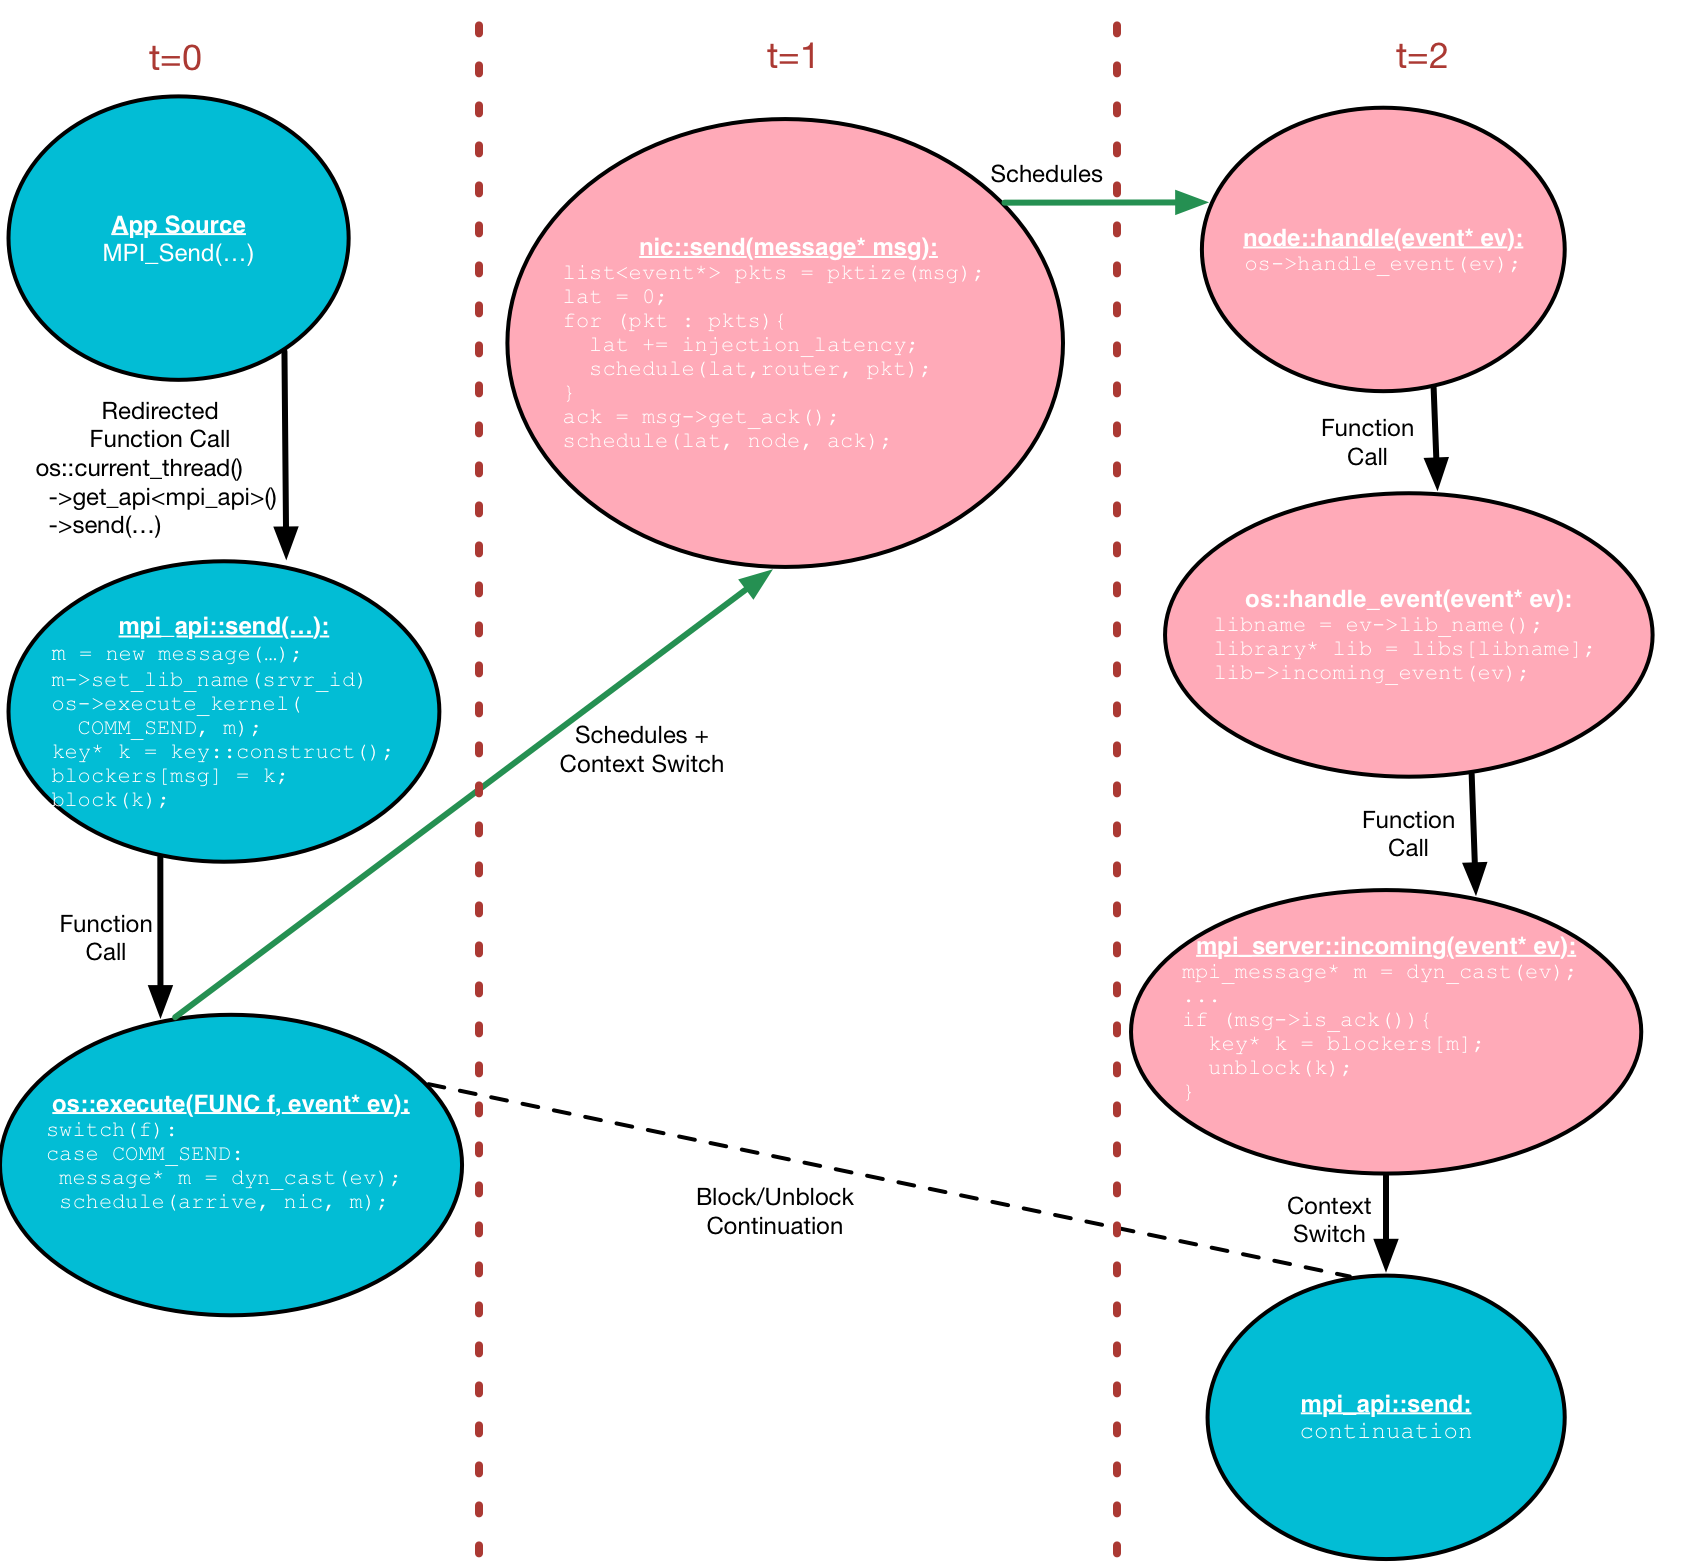
\includegraphics[width=1.05\textwidth]{figures/DES}
\caption{Flow of events for completing a send operation.  Shows basic function calls, block/unblock context switches, and event schedules. User-space thread (application) operations are shown in blue. Main event thread (OS/kernel) operations are shown in pink.}
\label{fig:desThreadsMPISend}
\end{figure}

When the ACK arrives back from the NIC, the ACK signals to MPI that the operation is complete allowing it to unblock.
The ACK is handled by a \inlinecode{service} object (which is the SST-specific implementation of an MPI server). 
A \inlinecode{service} is a special type of object, that we will discuss in more detail below.

\subsection{Thread-specific storage}
\label{subsec:threadStorage}
Let us look at the capture of the \inlinecode{MPI_Send} call. 
First, a macro redefines the call to avoid symbol clashes if using an MPI compiler (both virtual and real MPI cannot share symbols).
MPI uses global function calls to execute, meaning MPI has to operate on global variables.
However, SST/macro cannot use global variables.
Thus all state specific to each MPI rank (virtual thread) must be stashed somewhere unique.
This basically means converting all global variables into user-space thread-local variables.
When each user-space thread is spawned a \inlinecode{thread} object is allocated and associated with the thread.
This object acts as a container for holding all state specific to that virtual thread.
Rather than store MPI state in global variables, MPI state in stored in a class \inlinecode{mpi_api}, 
with one \inlinecode{mpi_api} object allocated per virtual MPI rank.
The operating system class provides a static function \inlinecode{current_thread} that makes the leap from
global variables to thread-local storage.
To access a specific API, a special helper template function \inlinecode{get_api} exists on each thread object.
Thus, instead of calling a global function \inlinecode{MPI_Send},
SST/macro redirects to a member function \inlinecode{send} on an \inlinecode{mpi_api} object that is specific to a virtual MPI rank.

\begin{table}
\def\arraystretch{1.5}
\begin{tabular}{>{\raggedright}p{2cm} >{\raggedright}p{3cm} >{\raggedright}p{3cm} >{\raggedright}p{3cm} >{\raggedright\arraybackslash}p{3cm}}
\hline
 & OS & Node & API & Service \\
\hline
Runs on Thread & 
  Both user-space and main DES thread &
  Only main DES thread (user-space with rare exceptions for optimization) &
%  Only main DES thread &
  Only user-space thread &
  Only main DES thread \\
How Advances Time & 
  Both blocking and scheduling events, depending on context &
  Scheduling events to other components &
%  Scheduling events to other components &
  Blocking or unblocking &
  Scheduling events to other components \\
Receives Events Via &
  Function calls from API/Service or from Node via \inlinecode{handle_event} function &
  Function calls from OS, receives scheduled events via the \inlinecode{handle} function &
%  Function calls from Node, receives scheduled events via \inlinecode{handle} function &
  Does not usually receive events - only blocks or unblocks &
  OS forwards messages to \inlinecode{incoming_event} function \\
Sends Events Via &
  Makes function calls and schedules events to Node &
  Makes function calls and schedules events to NIC, Memory &
%  Schedules events to Node, Interconnect &
  Does not usually send events - only blocks or unblocks &
  Makes function calls and schedules events to OS, unblocks APIs
\end{tabular}
\end{table}

\section{Libraries}
\label{sec:libraries}
The creating and handling of software events is managed through \inlinecode{library} objects.
Each \inlinecode{node} has an \inlinecode{operating_system} member variable that will manage software events on a virtual compute node.
Each library object is stored in a lookup table in the operating system,
allowing the operating system to access specific libraries at specific times.

\begin{CppCode}
class operating_system {
  ...
  map<string,library*> libs_;
  ...
};
\end{CppCode}

Each library object has access to the operating system, being allowed to call

\begin{CppCode}
event* ev = ...
os_->execute_kernel(ty, ev);
\end{CppCode}
or possibly 

\begin{CppCode}
event* ev = ...
os_->execute(ty, ev);
\end{CppCode}
where an enum argument \inlinecode{ty} specifies the type of computation or communication and the event object carries all the data needed to model it.
This allows a library to \emph{call out} to the operating system.
Calls to \inlinecode{execute} \emph{always} occur on a user-space thread. 
In executing a computation or communication, the operating system may block inside \emph{execute} to advance time to complete the operation.
Calls to \inlinecode{execute_kernel} can occur on either a user-space thread or the main event thread.
Here the operating system acts as a service and \emph{never} blocks.

Conversely, each \inlinecode{library} must provide a \inlinecode{incoming_event} method that allows the operating system to call back to the library

\begin{CppCode}
void incoming_event(event* ev){...}
\end{CppCode}
Generally speaking, event notifications will arrive from the NIC (new messages, ACKs), memory system (data arrived), processor (computation complete), etc.
These hardware events must be routed to the correct software library for processing.

The operating system provides an abstract interface (independent of the exact implementation of threading library) through \inlinecode{key} objects.
Each blocking call:

\begin{CppCode}
key* k = key::construct();
os->block(k);
\end{CppCode}

must be matched with a corresponding unblock on the same key object.
Usually libraries stash keys in some sort of lookup table to track event completions.

\begin{CppCode}
key* k = blockers[ev->uid()];
os->unblock(k);
\end{CppCode}

\begin{CppCode}
void
operating_system::handle_event(event* ev) {
  library* lib = libs_[ev->lib_name()];
  lib->incoming_event(ev);
}
\end{CppCode}
In order to route events to the correct library, the operating system maintains a string lookup table of \inlinecode{library} objects.
All events associated with that library must be constructed with the correct string label, 
accessible through the event accessor function \inlinecode{lib_name}.

\subsection{API}
\label{subsec:softwareAPI}
The SST/macro definition of API was alluded to in \ref{subsec:threadStorage}.
The base \inlinecode{api} class inherits from \inlinecode{library}.
All API code must execute on a user-space thread.
API calls are always associated with a specific virtual MPI rank.
To advance time, API calls must block and unblock.
Functions executing on user-space threads are ``heavyweight'' in the sense that they consume resources.
API compute calls must allocate cores via a compute scheduler to execute.


API objects are accessible in skeleton apps through a global template function is provided in \inlineshell{sstmac/skeleton.h}.

\begin{CppCode}
template <class T>
T* get_api();
\end{CppCode}
for which the implementation is

\begin{CppCode}
thread* thr = operating_system::current_thread();
return thr->get_api<T>();
\end{CppCode}
which converts the global template function into a thread-specific accessor.
The most prominent example of an API is the \inlinecode{mpi_api} object for encapsulating an MPI rank.
Other prominent examples include the various computation APIs such as \inlinecode{blas_api} that provides bindings for simulation various linear algebra functions.


\subsection{Service}
\label{subsec:service}
In contrast to an API that always executes on a user-space, services always execute on the main event thread.
They therefore never block (or unblock).
Services do not perform compute-heavy operations and therefore, in a simulator approximation, do not consume resources. 
For software to advance time, it must block and then unblock after a virtual time delay.
Services therefore have no ability to advance time and therefore all service operations are ``instantaneous.''
Again, this is an approximation for the sake of simulation simplicity and efficiency.
While an API can have several instances on a node (e.g. several MPI ranks on the same compute node), services are generally unique.
Examples of services are MPI or filesystem services that sort messages arriving from the NIC and pass them off to the correct API or library object.
If a service is ``heavy-weight'' and must model computational delays,
it must run as a full thread with its own user-space thread stack.

\section{Distributed Service}
\label{sec:distService}
In many cases, a service is just local to a node and is part of the operating system or a runtime library, such as a local filesystem or a server receiving incoming network messages.  In cases of something like a distributed file system like LUSTRE or distributed key-value store like Memcached, a service spans multiple nodes.  These services are much like skeleton applications in that they require a parallel launch with node allocation and rank indexing.

To create a new distributed service, you have to inherit from \inlinecode{sstmac::distributed_service} in \\
\inlineshell{sstmac/libraries/sumi/distributed_service.h}.  
Distributed services require a network transport layer to communicate between service nodes.
In contrast to other libraries and services that are found in \inlineshell{sstmac/software}, distributed services are linked to SUMI (SST unified message interface).
A distributed service must implement the \inlinecode{void run()} virtual member function.
In general, the \inlinecode{run} function will almost always perform something like:

\begin{CppCode}
void example_service::run()
{
 //some init
 bool block  = true;
 message::ptr msg = poll_for_message(block);
 while (msg && !terminated()){
   process(msg);
   msg = poll_for_message(block);
 }
}
\end{CppCode}
The function \inlinecode{poll_for_message} goes into a network polling loop looking for incoming messages.
Depending on the boolean parameter, the function will block until a message arrives or returns immediately if no message is available.
The service may receive a terminate message.
This gets processed automatically.
Whether a shutdown message has been received can be queried for by the \inlinecode{terminated} function.

Launching a distributed service is very similar to launching an application with a few subtle differences.
The services to be launched are listed in the input file as:

\begin{ViFile}
services = insitu_viz filesystem
\end{ViFile}
As a space-separated list.
This would launch services registered using the standard sprockit registration:

\begin{CppCode}
SpktRegister("filesystem", distributed_service, test_filesystem);
\end{CppCode}
The launch parameters and any service-specific parameters are done exactly as for applications, but go in a namespace corresponding to the service:

\begin{ViFile}
filesystem.launch_cmd = aprun -n 10 -N 1
filesystem.allocation = first_available
filesystem.reed_solomon_k = 5
filesystem.reed_solomon_n = 7
...
\end{ViFile}
This launches ten filesystem service nodes using a given node allocation strategy.
Some filesystem-specific parameters are given (in this case dealing with Reed-Solomon protection codes).

\subsection{Coordinating servers and clients}
\label{subsec:coordinatingServersClients}
Slightly more complicated is the process of communicating between service and client applications.
In many HPC simulations, the only thing being simulated is a single MPI application.
The default \inlinecode{send} function in \inlinecode{sumi_transport} assumes messages are being sent \emph{within} a given application.

\begin{CppCode}
void
send_payload(int dst, 
  const message::ptr& msg, 
  bool needs_ack);
\end{CppCode}
The only thing that must be specified is a destination \emph{rank}, which is the virtual ID within a given session layer.
The transport layer itself will map that to the correct physical node address and deliver the message.

An alternative function exists for sending from client to server:

\begin{CppCode}
void client_server_send(
  int dest_rank,
  node_id dest_node,
  app_id dest_app,
  const sumi::message::ptr& msg);
\end{CppCode}
While a session rank must be given, a physical node ID and an application ID must be given.
These can no longer be filled in automatically.

For a client to get all of the information about a distributed service, a special object is supplied that can be fetched:

\begin{CppCode}
sstmac::sw::app_launch* srv = sstmac::sw::app_launch::service_info("filesystem");
\end{CppCode}
The object \inlinecode{srv} has functions that can be queried to figure out all the \inlinecode{client_server_send} parameters.  
The parameter to the static \inlinecode{service_info} function is the service name given to \inlinecode{SpktRegister} and given in the input file.

The same \inlinecode{client_server_send} function is used for both clients making requests to servers and servers returning responses to clients.
In most cases, the clients will use \inlinecode{service_info} to ``discover'' the servers.
In order to receive responses, the clients should send messages containing all the relevant info with rank, physical node ID, and app ID.

Generally, an application knowns when it is done (e.g. reaches some convergence criterion). 
A service does not usually have a clean termination condition since it never knows when more client requests may arrive.
In this case, the function \inlinecode{shutdown_server} can be called by a client application.

\begin{CppCode}
void shutdown_server(
  int dest_rank,
  node_id dest_node,
  app_id dest_app);
\end{CppCode}

A single shutdown message to any server is sufficient to bring down the entire service.
The shutdown message will be automatically broadcast to all other nodes.

%\section{Computation}

%\subsection{Compute Events}

%\subsection{Timed Compute}

%\subsection{Performance Counters}


% !TEX root = developer.tex

\newcommand{\nodecls}{\inlinecode{node}\xspace}
\newcommand{\topcls}{\inlinecode{topology}\xspace}
\newcommand{\switchid}{\inlinecode{switch_id}\xspace}
\newcommand{\nodeid}{\inlinecode{node_id}\xspace}

\chapter{Hardware Models}
\label{chapter:hardware}

\section{Overview}
To better understand how hardware models are put together for simulating interconnects, we should try to understand the basic flow of event in SST/macro involved in sending a message between two network endpoints.  We have already seen in skeleton applications in previous sections how an application-level call to a function like \inlinecode{MPI_Send} is mapping to an operating system function and finally a hardware-level injection of the message flow.  Overall, the following steps are required:

\begin{enumerate}
\item Start message flow with app-level function call
\item Push message onto NIC for send
\item NIC packetizes message and pushes packets on injection switch
\item Packets are routed and traverse the network
\item Packets arrive at destination NIC and are reassembled (potentially out-of-order)
\item Message flow is pushed up network software stack
\end{enumerate}

Through the network, packets must move through buffers (waiting for credits) and arbitrate for bandwidth through the switch crossbar and then through the ser/des link on the switch output buffers.  The control-flow diagram for transporting a flow from one endpoint to another via packets is shown in Figure \ref{fig:controlFlow}

\begin{figure}
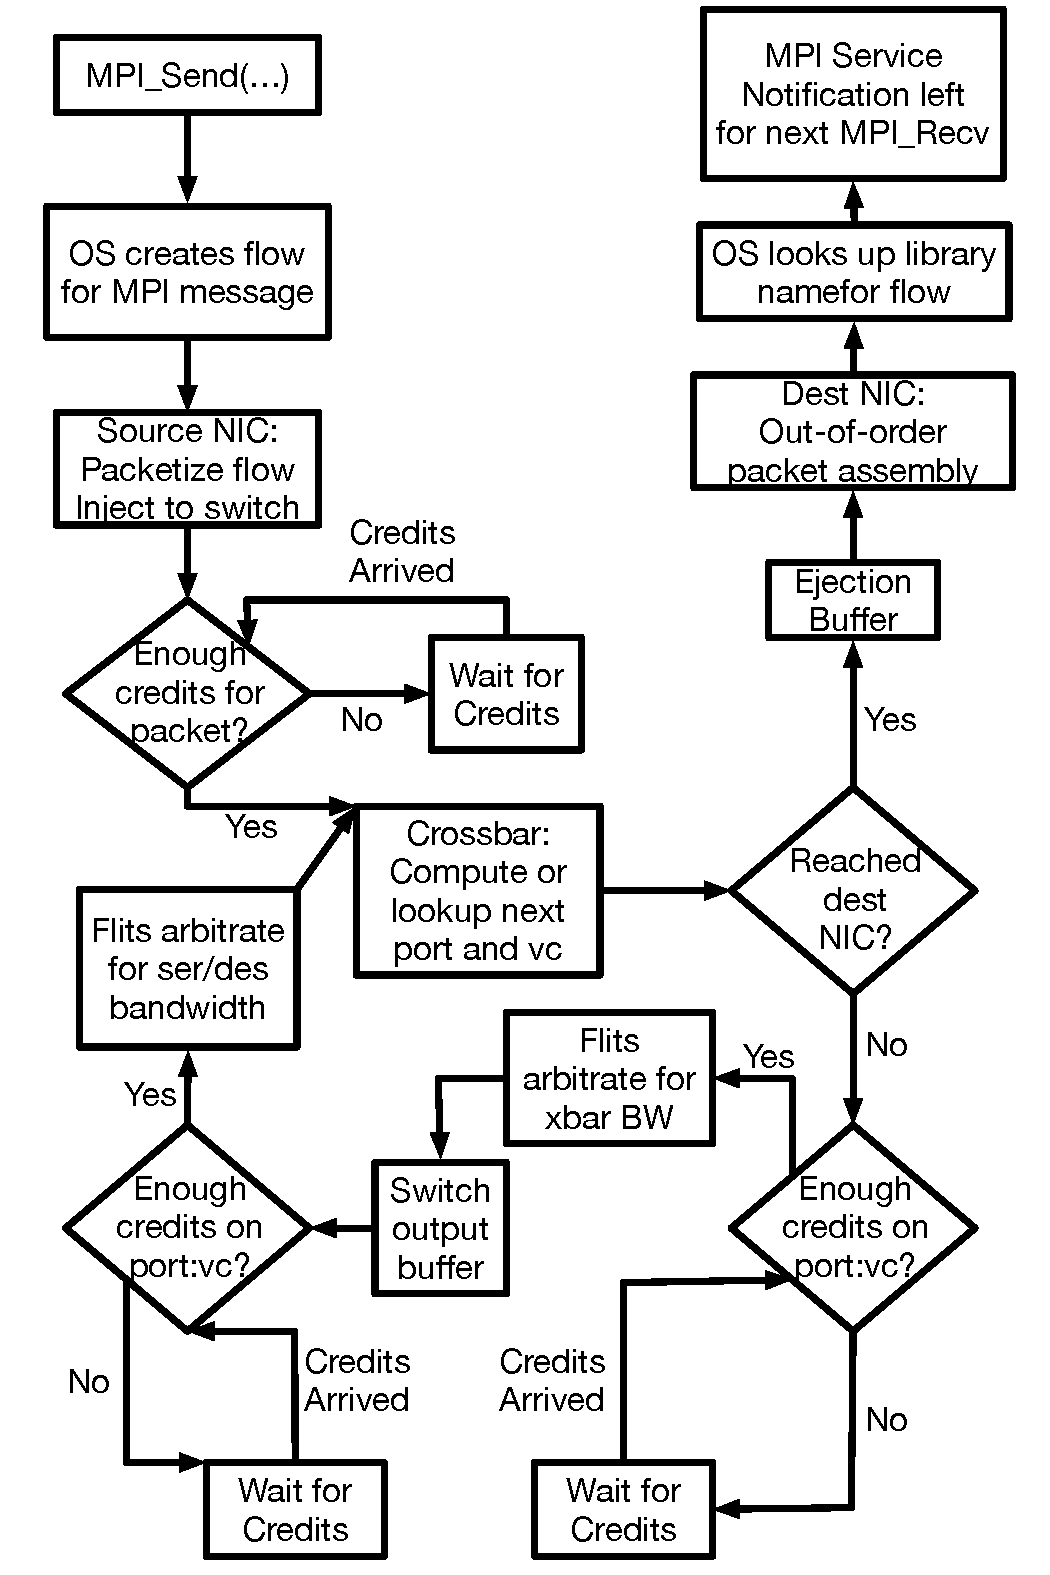
\includegraphics[width=0.8\textwidth]{figures/DecisionFlow}
\caption{Decision diagram showing the various control flow operations that occur as a message is transport across the network via individual packet operations.}
\label{fig:controlFlow}
\end{figure}

We can dive in deeper to the operations that occur on an individual component, mostly important the crossbar on the network switch. Figure \ref{fig:xbarFlow} shows code and program flow for a packet arriving at a network switch.  The packet is routed (virtual function, configurable via input file parameters), credits are allocated to the packet, and finally the packet is arbitrated across the crossbar. After arbitration, a statistics callback can be invoked to collect any performance metrics of interest (congestion, traffic, idle time).

\begin{figure}
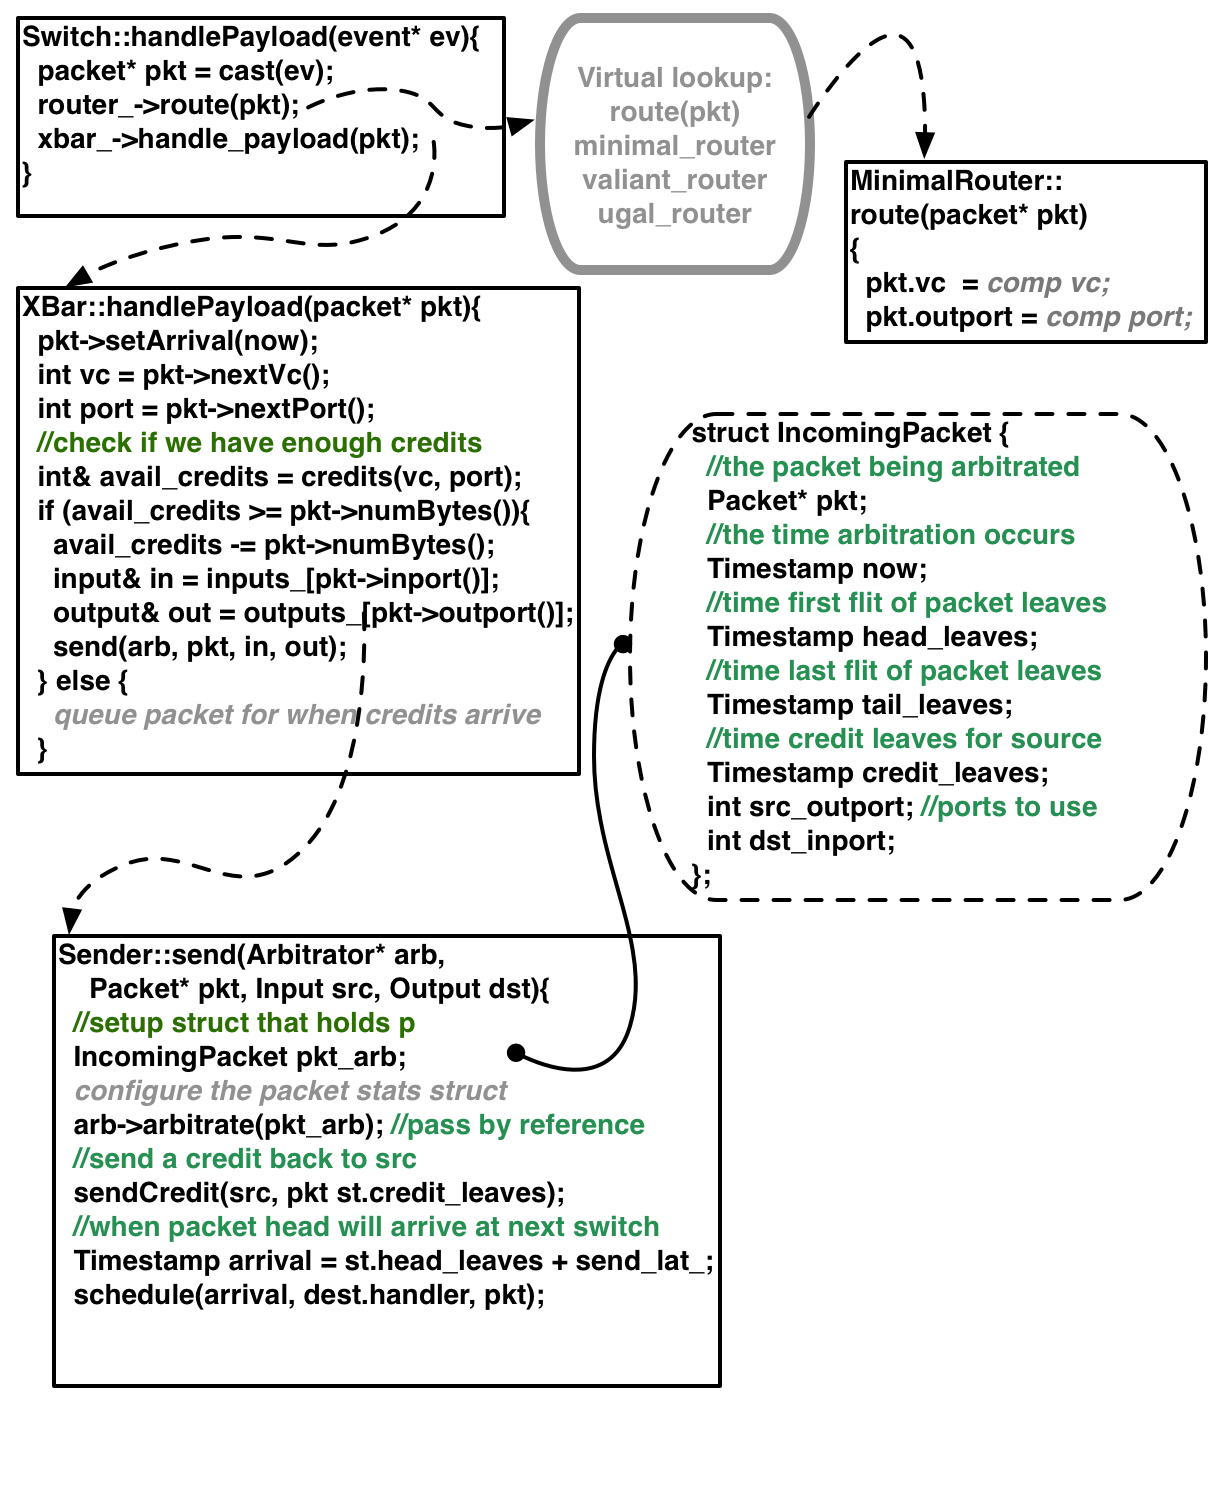
\includegraphics[width=0.9\textwidth]{figures/RoutingFlow}
\caption{Code flow for routing, arbitration, and stats collections of packets traversing the crossbar on the network switch.}
\label{fig:xbarFlow}
\end{figure}

\section{Connectables}
\label{sec:connectables}
With a basic overview of how the simulation proceeds, we can now look at the actual SST/macro class types.
While in common usage, \sstmacro follows a well-defined machine model (see below),
it generally allows any set of components to be connected. 
As discussed in Chapter \ref{chapter:des}, the simulation proceeds by having event components exchange messages,
each scheduled to arrive at a specific time.
\sstmacro provides a generic interface for any set of hardware components to be linked together.
Any hardware component that connects to other components and exchanges messages must inherit from the \inlinecode{connectable} class.
The \inlinecode{connectable} class presents a standard virtual interface

\begin{CppCode}
class connectable
{
 public:
  virtual void
  connect_output(
    sprockit::sim_parameters* params,
    int src_outport,
    int dst_inport,
    connectable* mod,
    event_handler* handler) = 0;

  virtual void
  connect_input(
    sprockit::sim_parameters* params,
    int src_outport,
    int dst_inport,
    connectable* mod,
    event_handler* handler) = 0;


};
\end{CppCode}

First, port numbers must be assigned identifying the output port at the source and in the input port at the destination.
For example, a switch may have several outgoing connections, each of which must be assigned a unique port number.
The connection must be configured at both source and destination.
The function is called twice for each side of the connection. If we have a source and destination:

\begin{CppCode}
connectable* src = ...
connectable* dst = ...
sprockit::sim_parameters* params = ...
src->connect_output(params, inport, outport, Output, dst);
dst->connect_input(params, inport, outport, Input, src);
\end{CppCode}

A certain style and set of rules is recommended for all connectables.
If these rules are ignored, setting up connections can quicky become confusing and produce difficult to maintain code.
The first and most important rule is that \inlinecode{connectables} never make their own connections.
Some ``meta''-object should create connections between objects.
In general, this work is left to a \inlinecode{interconnect} object.
An object should never be responsible for knowing about the ``world'' outside itself.
A topology or interconnect tells the object to make a connection rather than the object deciding to make the connection itself.
This will be illustrated below in \ref{sec:topology}.

The second rule to follow is that a connect function should never call another connect function.
In general, a single call to a connect function should create a single link.
If connect functions start calling other connect functions, you can end up a with a recursive mess.
If you need a bidirectional link (A $\rightarrow$ B, B $\rightarrow$ A),
two separate function calls should be made

\begin{CppCode}
A->connect_output(B);
B->connect_input(A);
\end{CppCode}

rather than having, e.g. A create a bidirectional link.

The first two rules should be considered rigorous. 
A third recommended rule is that all port numbers should be non-negative, and, in most cases, should start numbering from zero.


Combining the factory system for polymorphic types and the connectable system for building arbitrary machine links and topologies,
\sstmacro provides flexibility for building essentially any machine model you want.
However, \sstmacro provides a recommended machine structure to guide constructing machine models.

\section{Interconnect}\label{sec:topInterconnect}
For all standard runs, the entire hardware model is driven by the interconnect object.
The interconnect creates nodes, creates network switches, chooses a topology, and connects all of the network endpoints together.
In this regard, the interconnect also choose what types of components are being connected together.
For example, if you were going to introduce some custom FPGA device that connects to the nodes to perform filesystem operations,
the interconnect is responsible for creating it.

To illustrate, here is the code for the interconnect that creates the node objects. 
The interconnect is itself a factory object, configured from a parameter file.

\begin{CppCode}
interconnect::interconnect(sprockit::sim_parameters* params, event_manager* mgr, partition* part, parallel_runtime* rt)
{
  sprockit::sim_parameters* top_params = params->get_namespace("topology");
  topology_ = topology_factory::get_param("name", top_params);
  num_nodes_ = topology_->num_nodes();
  num_switches_ = topology_->num_switches();
  
  switches_.resize(num_switches_);
  nodes_.resize(num_nodes_);

  sprockit::sim_parameters* node_params = params->get_namespace("node");
  sprockit::sim_parameters* switch_params = params->get_namespace("switch");
  
  sprockit::sim_parameters* nic_params = node_params->get_namespace("nic");
  sprockit::sim_parameters* inj_params = nic_params->get_namespace("injection");
  sprockit::sim_parameters* ej_params = switch_params->get_namespace("ejection"); 
  
  build_endpoints(node_params, nic_params, mgr);
  build_switches(switch_params, mgr);
  connect_endpoints(inj_params, ej_params);
  connect_switches(switch_params); 
}
\end{CppCode}

For full details of the functions that build/connect endpoints and switches, consult the source code.
In general, the \inlinecode{interconnect} object uses the connectable interface to setup all the connections.
It uses the topology interface to determine which connections are required, e.g.

\begin{CppCode}
switch_id src = ...
std::vector<topology::connection> outports;
topology_->connected_outports(src, outports);
for (auto& conn : outports){
  network_switch* dst_sw = switches_[conn.dst];
  src_sw->connect_output(params, conn.src_outport, conn.dst_inport,
  					 dst_sw->payload_handler(conn.dst_inport));
  dst_sw->connect_input(params, conn.src_outport, conn.dst_inport,
  				       src_sw->ack_handler(conn.src_outport));
}
\end{CppCode}
The \inlinecode{connected_outports} function takes a given source switch and returns all the connections that the
switch is supposed to make.  Each switch must provide \inlinecode{payload_handler} and \inlinecode{ack_handler} functions to return
the \inlinecode{event_handler} that should receive either new packets (payload) or credits (ack) for the connections.

\section{Node}\label{sec:node}
Although the \nodecls can be implemented as a very complex model, it fundamentally only requires a single set of functions to meet the public interface.
The \nodecls must provide \inlinecode{execute_kernel} functions that are invoked by the \inlinecode{operating_system} or other other software objects.
The prototypes for these are:

\begin{CppCode}
virtual void
execute(ami::COMP_FUNC func, event* data);

virtual void
execute(ami::SERVICE_FUNC func, event* data);
\end{CppCode}	

By default, the abstract \nodecls class throws an \inlinecode{sprockit::unimplemented_error}. These functions are not pure virtual.
A node is only required to implement those functions that it needs to do.
The various function parameters are enums for the different operations a node may perform:
computation or communication. Computation functions are those that require compute resources. Service functions are special functions that run in the background and ``lightweight'' such that any modeling of processor allocation should be avoided. Service functions are run ``for free'' with no compute 

\section{Network Interface (NIC)}\label{sec:nic}
The network interface can implement many services, but the basic public interface requires the NIC to do three things:

\begin{itemize}
\item Inject messages into the network
\item Receive messages ejected from the network
\item Deliver ACKs (acknowledgments) of message delivery
\end{itemize}

For sending messages, the NIC must implement

\begin{CppCode}
  virtual void
  do_send(network_message* payload);
\end{CppCode}
A non-virtual, top-level \inlinecode{send} function performs operations standard to all NICs.
Once these operations are complete, the NIC invokes \inlinecode{do_send} to perform model-specific send operations.
The NIC should only ever send \inlinecode{network_message} types.

For the bare-bones class \inlinecode{logp_nic}, the function is

\begin{CppCode}
void
logp_nic::do_send(network_message* msg)
{
  long num_bytes = msg->byte_length();
  timestamp now_ = now();
  timestamp start_send = now_ > next_free_ ? now_ : next_free_;
  timestamp time_to_inject = inj_lat_ + timestamp(inj_bw_inverse_ * num_bytes);
  //leave the injection latency term to the interconnect
  schedule_now(injection_switch_, msg);

  next_free_ = start_send + time_to_inject;
  if (msg->needs_ack()) {
    //do whatever you need to do so that this msg decouples all pointers
    network_message* acker = msg->clone_injection_ack();
    schedule(next_free_, parent_->self_handler(), acker); //send to node
  }
}
\end{CppCode}
After injecting, the NIC creates an ACK and delivers the notification to the \nodecls.
In general, all arriving messages or ACKs should be delivered to the node.
The node is responsible for generating any software events in the OS.

For receiving, messages can be moved across the network and delivered in two different ways:
either at the byte-transfer layer (BTL) or message-transfer layer (MTL).
Depending on the congestion model, a large message (say a 1 MB MPI message) might be broken up into many packets.
These message chunks are moved across the network independently and then reassembled at the receiving end.
Alternatively, for flow models or simple analytical models, the message is not packetized and instead delivered as a single whole.
The methods are not pure virtual.  Depending on the congestion model,  the NIC might only implement chunk receives or whole receives.
Upon receipt, just as for ACKs, the NIC should deliver the message to the node to interpret.
In general, \inlinecode{nic::handle} is intended to handle packets. 
If a NIC supports direct handling of complete messages (MTL) instead of packets (BTL),
it should provide a message handler:

\begin{CppCode}
event_handler*
mtl_handler() const {
  return mtl_handler_;
}
\end{CppCode}

A special completion queue object tracks chunks and processes out-of-order arrivals,
notifying the NIC when the entire message is done.

\section{Memory Model}\label{sec:memModel}
As with the NIC and node, the memory model class can have a complex implementation under the hood,
but it must funnel things through the a common function.

\begin{CppCode}
virtual void
access(long bytes, double max_bw) = 0;
\end{CppCode}

This function is intended to be called from an application user-space thread.
As such, it should block until complete.
For more details on the use of user-space threading to model applications,
see the User's manual.


\section{Network Switch}\label{sec:networkSwitch}

Unlike the other classes above, a network switch is not required to implement any specific functions.
It is only required to be an \inlinecode{event_handler}, providing the usual \inlinecode{handle(event* ev)}.
The internal details can essentially be arbitrary.
However, the basic scheme for most switches follows the code below for the \inlinecode{packet_flow} model.

\begin{CppCode}
void
packet_flow_switch::handle_credit(event *ev)
{
  packet_flow_credit* credit = static_cast<packet_flow_credit*>(ev);
  out_buffers_[credit->port()]->handle_credit(credit);
}

void
packet_flow_switch::handle_payload(event *ev)
{
  packet_flow_payload* payload = static_cast<packet_flow_payload*>(ev);
  router_->route(payload);
  xbar_->handle_payload(payload);
}
\end{CppCode}
The arriving event is sent to either a credit handler or a payload handler,
which is configured during simulation setup.
If a packet, the router object selects the next destination (port).
The packet is then passed to the crossbar for arbitration.

\section{Topology}
\label{sec:topology}
Of critical importance for the network modeling is the topology of the interconnect.
Common examples are the torus, fat tree, or butterfly.
To understand what these topologies are, there are many resources on the web.
Regardless of the actual structure as a torus or tree, the topology should present a common interface to the interconnect and NIC for routing messages.
Here we detail the public interface.
\subsection{Basic Topology}
Not all topologies are ``regular'' like a torus.  Ad hoc computer networks (like the internet) are ordered with IP addresses, but don't follow a regular geometric structure.
The abstract topology base class is intended to cover both cases.
Irregular or arbitrary topology connections are not fully supported yet.

The most important functions in the \topcls class are

\begin{CppCode}
class topology
{
virtual bool
uniform_network_ports() const = 0;

virtual bool
uniform_switches_non_uniform_network_ports() const = 0;

virtual bool
uniform_switches() const = 0;

virtual void
connected_outports(switch_id src, std::vector<topology::connection>& conns) const = 0;

virtual void
configure_individual_port_params(switch_id src,
      sprockit::sim_parameters* switch_params) const = 0;

virtual int
num_switches() const = 0;

virtual int
num_leaf_switches() const = 0;

virtual int
num_nodes() const = 0;

virtual int
num_endpoints() const = 0;

virtual int
max_num_ports() const = 0;

virtual switch_id
endpoint_to_injection_switch(node_id nodeaddr, int& switch_port) const = 0;

virtual switch_id
endpoint_to_ejection_switch(node_id nodeaddr, int& switch_port) const = 0;

virtual void
configure_vc_routing(std::map<routing::algorithm_t, int>& m) const = 0;

virtual switch_id
node_to_ejection_switch(node_id addr, int& port) const = 0;

virtual int
minimal_distance(switch_id src, switch_id dst) const = 0;

virtual int
num_hops_to_node(node_id src, node_id dst) const = 0;

virtual void
nodes_connected_to_injection_switch(switch_id swid,
                      std::vector<injection_port>& nodes) const = 0;

virtual void
nodes_connected_to_ejection_switch(switch_id swid,
                      std::vector<injection_port>& nodes) const = 0;

virtual void
minimal_route_to_switch(
switch_id current_sw_addr,
switch_id dest_sw_addr,
routable::path& path) const = 0;

virtual bool
node_to_netlink(node_id nid, node_id& net_id, int& offset) const = 0;
\end{CppCode}

These functions are documented in the \inlineshell{topology.h} header file.
The first few functions just give the number of switches, number of nodes, and finally which nodes are connected to a given switch.
Each compute node will be connected to an injector switch and an ejector switch (often the same switch).
The topology must provide a mapping between a node and its ejection and injection points.
Additionally, the topology must indicate a port number or offset for the injection in case the switch has many nodes injecting to it.
The most important thing to distinguish here are \nodeid and \switchid types.
These are typedefs that distinguish between a switch in the topology and a node or network endpoint.

Besides just forming the connections, a topology is responsible for routing.
Given a source switch and the final destination, a topology must fill out path information.

\begin{CppCode}
struct path {
    int outport;
    int vc;
    int geometric_id;
    sprockit::metadata_bits<uint32_t> metadata;
}
\end{CppCode}

The most important information is the outport, telling a switch which port to route along to arrive at the destination.
For congestion models with channel dependencies, the virtual channel must also be given to avoid deadlock.
In general, network switches and other devices should be completely topology-agnostic.
The switch is responsible for modeling congestion within itself - crossbar arbitration, credits, outport multiplexing.
The switch is not able to determine for itself which outport to route along.
The topology tells the switch which port it needs and the switch determines what sort of congestion delay to expect on that port.
This division of labor is complicated a bit by adaptive routing, but remains essentially the same.  More details are given later.

\section{Router}\label{sec:router}
The router has a simple public interface

\begin{CppCode}
class router
{
...
  virtual void
  route(packet* pkt);

  virtual void
  route_to_switch(switch_id sid, routable::path& path) = 0;
...
};
\end{CppCode}

Different routers exist for the different routing algorithms: 	minimal, valiant, ugal.
The router objects are specific to a switch and can therefore store state information.
However, the router should query the topology object for any path-specific information, e.g.

\begin{CppCode}
void
minimal_router::route_to_switch(switch_id sid, routable::path& path)
{
  top_->minimal_route_to_switch(my_addr_, sid, path);
}
\end{CppCode}

For adaptive routing, a bit more work is done.
Each router is connect to a switch object which holds all the information about queue lengths, e.g.

\begin{CppCode}
int test_length = get_switch()->queue_length(paths[i].outport);
\end{CppCode}
allowing the router to select an alternate path if the congestion is too high. 



% !TEX root = developer.tex

\chapter{A Custom Object: Beginning To End}
\label{chapter:custom}

Suppose we have brilliant design for a new topology we want to test.
We want to run a simple test \emph{without} having to modify the \sstmacro build system.
We can create a simple external project that links the new topology object to \sstmacro libraries.
The Makefile can be found in \inlineshell{tutorials/programming/topology}.
You are free to make \emph{any} Makefile you want.
After \sstmacro installs, it creates compiler wrappers \inlineshell{sst++} and \inlineshell{sstcc}
in the chosen \inlineshell{bin} folder.  
These are essentially analogs of the MPI compiler wrappers.
This configures all include and linkage for the simulation.

We want to make an experimental topology in a ring.
Rather than a simple ring with connections to nearest neighbors, though, we will have ``express'' connections that jump to switches far away.

We begin with the standard typedefs.
\begin{CppCode}
#include <sstmac/hardware/topology/structured_topology.h>

namespace sstmac {
namespace hw {

class xpress_ring :
  public structured_topology
{
 public:
  typedef enum {
    up_port = 0,
    down_port = 1,
    jump_up_port = 2,
    jump_down_port = 3
  } port_t;

  typedef enum {
    jump = 0, step = 1
  } stride_t;

\end{CppCode} 
Packets can either go to a nearest neighbor or they can ``jump'' to a switch further away.
Each switch in the topology will need four ports for step/jump going up/down.
The header file can be found in \inlineshell{tutorials/programm/topology/xpressring.h}.
We now walk through each of the functions in turn in the source in the topology public interface.
We got some functions for free by inheriting from \inlinecode{structured_topology}.

We start with

\begin{CppCode}
void
xpress_ring::init_factory_params(sprockit::sim_parameters* params)
{
  structured_topology::init_factory_params(params);
  ring_size_ = params->get_int_param("xpress_ring_size");
  jump_size_ = params->get_int_param("xpress_jump_size");
}
\end{CppCode}
determining how many switches are in the ring and how big a ``jump'' link is.

The topology then needs to tell objects how to connect

\begin{CppCode}
void
xpress_ring::connect_objects(connectable_map& objects)
{
  for (int i=0; i < ring_size_; ++i) {
    connectable* center_obj = objects[switch_id(i)];

    switch_id up_idx((i + 1) % ring_size_);
    connectable* up_partner = find_object(objects, cloner, up_idx);
    center_obj->connect(up_port, down_port, connectable::network_link, up_partner);

    switch_id down_idx((i + ring_size_ - 1) % ring_size_);
    connectable* down_partner = find_object(objects, cloner, down_idx);
    center_obj->connect_mod_at_port(down_port, up_port, connectable::network_link,
                                    down_partner);

    switch_id jump_up_idx((i + jump_size_) % ring_size_);
    connectable* jump_up_partner = find_object(objects, cloner, jump_up_idx);
    center_obj->connect(jump_up_port, jump_down_port, connectable::network_link,
                                    jump_up_partner);

    switch_id jump_down_idx((i + ring_size_ - jump_size_) % ring_size_);
    connectable* jump_down_partner = find_object(objects, cloner,
                                         jump_down_idx);
    center_obj->connect(jump_down_port, jump_up_port, connectable::network_link,
                                    jump_down_partner);
  }
}
\end{CppCode}
We loop through every switch in the ring and form $+/-$ connections to neighbors and $+/-$ connections to jump partners.
Each of the four connections get a different unique port number.  We must identify both the outport port for the sender and the input port for the receiver.

To compute the distance between two switches

\begin{CppCode}
int
xpress_ring::num_hops(int total_distance) const
{
  int num_jumps = total_distance / jump_size_;
  int num_steps = total_distance % jump_size_;
  int half_jump = jump_size_ / 2;
  if (num_steps > half_jump) {
    //take an extra jump
    ++num_jumps;
    num_steps = jump_size_ - num_steps;
  }
  return num_jumps + num_steps;
}

int
xpress_ring::minimal_distance(
  const coordinates& src_coords,
  const coordinates& dest_coords) const
{
  int src_pos = src_coords[0];
  int dest_pos = dest_coords[0];
  int up_distance = abs(dest_pos - src_pos);
  int down_distance = abs(src_pos + ring_size_ - dest_pos);

  int total_distance = std::max(up_distance, down_distance);
  return num_hops(total_distance);
}
\end{CppCode}
Essentially you compute the number of jumps to get close to the final destination and then the number of remaining single steps.

For computing coordinates, the topology has dimension one.
\begin{CppCode}
switch_id
xpress_ring::get_switch_id(const coordinates& coords) const
{
  return switch_id(coords[0]);
}

void
xpress_ring::get_productive_path(
  int dim,
  const coordinates& src,
  const coordinates& dst,
  routing_info::path& path) const
{
  minimal_route_to_coords(src, dst, path);
}

void
xpress_ring::compute_switch_coords(switch_id swid, coordinates& coords) const
{
  coords[0] = int(swid);
}
\end{CppCode}
Thus the coordinate vector is a single element with the \switchid.

The most complicated function is the routing function.

\begin{CppCode}
void
xpress_ring::minimal_route_to_coords(
  const coordinates& src_coords,
  const coordinates& dest_coords,
  routing_info::path& path) const
{
  int src_pos = src_coords[0];
  int dest_pos = dest_coords[0];

  //can route up or down
  int up_distance = abs(dest_pos - src_pos);
  int down_distance = abs(src_pos + ring_size_ - dest_pos);
  int xpress_cutoff = jump_size_ / 2;
\end{CppCode}
First we compute the distance in the up and down directions.
We also compute the cutoff distance where it is better to jump or step to the next switch.
If going up is a shorter distance, we have

\begin{CppCode}
  if (up_distance <= down_distance) {
    if (up_distance > xpress_cutoff) {
      path.outport = jump_up_port;
      path.dim = UP;
      path.dir = jump;
      path.vc = 0;
    }
    else {
      path.outport = up_port;
      path.dim = UP;
      path.dir = step;
      path.vc = 0;
    }
  }
\end{CppCode}
We then decide if it is better to step or jump.
We do not concern ourselves with virtual channels here and just set it to zero.
Similarly, if the down direction in the ring is better

\begin{CppCode}
  else {
    if (down_distance > xpress_cutoff) {
      path.outport = jump_down_port;
      path.dim = DOWN;
      path.dir = jump;
      path.vc = 0;
    }
    else {
      path.outport = down_port;
      path.dim = DOWN;
      path.dir = step;
      path.vc = 0;
    }
  }
}
\end{CppCode}

For adaptive routing, we need to compute productive paths.
In this case, we only have a single dimension so there is little adaptive routing flexibility.
The only productive paths are the minimal paths.

\begin{CppCode}
void
xpress_ring::get_productive_path(
  int dim,
  const coordinates& src,
  const coordinates& dst,
  routing_info::path& path) const
{
  minimal_route_to_coords(src, dst, path);
}
\end{CppCode}

We are now ready to use our topology in an application.
In this case, we just demo with the built-in MPI ping all program from \sstmacro.
Here every node in the network sends a point-to-point message to every other node.
There is a parameter file in the \inlineshell{tutorials/programming/toplogy} folder.
To specify the new topology

\begin{ViFile}
# Topology
topology.name = xpress
topology.xpress_ring_size = 10
topology.xpress_jump_size = 5
\end{ViFile}
with application launch parameters

\begin{ViFile}
# Launch parameters
launch_indexing = block
launch_allocation = first_available
launch_app1_cmd = aprun -n10 -N1
launch_app1 = mpi_test_all
\end{ViFile}
The file also includes a basic machine model.

After compiling in the folder, we produce an executable \inlineshell{runsstmac}.
Running the executable, we get the following

\begin{ShellCmd}
Estimated total runtime of           0.00029890 seconds
SST/macro ran for       0.4224 seconds
\end{ShellCmd}
where the \sstmacro wall clock time will vary depending on platform.
We estimate the communication pattern executes and finishes in 0.30 ms.
Suppose we change the jump size to a larger number.
Communication between distant nodes will be faster, but communication between medium-distance nodes will be slower.
We now set \inlinefile{jump_size = 10} and get the output

\begin{ShellCmd}
Estimated total runtime of           0.00023990 seconds
SST/macro ran for       0.4203 seconds
\end{ShellCmd}
We estimate the communication pattern executes and finishes in 0.24 ms, a bit faster.
Thus, this communication pattern favors longer jump links.



% !TEX root = developer.tex

\chapter{How \sstmacro Launches}
\label{chapter:launching}

It is useful for an intuitive understanding of the code to walk through the steps starting from \inlinecode{main} and proceeding to the discrete event simulation actually launching. The code follows these basic steps:

\begin{enumerate}
\item Configuration of the simulation via environment variables, command line parameters, and the input file
\item Building and configuration of simulator components
\item Running of the actual simulation
\end{enumerate}

We can walk through each of these steps in more detail.

\section{Configuration of Simulation}\label{sec:simConfig}
The configuration proceeds through the following basic steps:
\begin{enumerate}
\item Basic initialization of the \inlinecode{parallel_runtime} object from environment variables and command line parameters
\item Processing and parallel broadcast of the input file parameters
\item Creation of the simulation \inlinecode{manager} object
\item Detailed configuration of the \inlinecode{manager} and \inlinecode{parallel_runtime} object

The first step in most programs is to initialize the parallel communication environment via calls to MPI\_Init or similar.
Only rank 0 should read in the input file to minimize filesystem traffic in a parallel job.
Rank 0 then broadcasts the parameters to all other ranks.
We are thus left with the problem of wanting to tune initialization of the parallel environment via the input file,
but the input file is not yet available.
Thus, we have an initial bootstrap step where the all parameters affecting initialization of the parallel runtime must be given
either via command line parameters or environment variables.
These automatically get distributed to all processes via the job launcher.
Most critically the environment variable \inlineshell{SSTMC_PARALLEL} takes on values of \inlineshell{serial} or \inlineshell{mpi}.

As stated above, only rank 0 ever touches the filesystem.
A utility is provided within the Sprockit library for automatically distributing files via the \inlinecode{parallel_build_params} function within \inlinecode{sim_parameters}.
Once broadcast, all ranks now have all they need to configure, setup, and run.
Some additional processing is done here to map parameters.
If parameters are missing, \sstmacro may fill in sensible defaults at this stage.
For deprecated parameters, \sstmacro also does some remapping to ensure backwards compatibility.

After creation of the \inlinecode{manager} object, 
since all of the parameters even from the input file are now available,
a more detailed configuration of the \inlinecode{manager} and \inlinecode{parallel_runtime} can be done.

\section{Building and configuration of simulator components}\label{sec:buildConfig}
Inside the function \inlinecode{mgr->init_factory_params},
the simulation manager now proceeds to build all the necessary components.
There are three basic classes of components to build.

\begin{itemize}
\item The event manager that drives the discrete event simulation
\item The interconnect object that directs the creation of all the hardware components
\item The generation of application objects that will drive the software events
\end{itemize}

\subsection{Event Manager}\label{sec:eventMan}
The \inlinecode{event_manager} object is a polymorphic type that depends on 1) what sort of parallelism is being used and 2) what sort of data structure is being used.
Some allowed values include \inlineshell{event_map} or \inlineshell{event_calendar} via the \inlineshell{event_manager} variable in the input file.
For parallel simulation, only the \inlineshell{event_map} data structure is currently supported.
For MPI parallel simulations, the \inlineshell{event_manager} parameter should be set to \inlineshell{clock_cycle_parallel}.
For multithreaded simulations (single process or coupled with MPI), this should be set to \inlineshell{multithread}.
In most cases, \sstmacro chooses a sensible default based on the configuration and installation.

As of right now, the event manager is also responsible for partitioning the simulation.
This may be refactored in future versions.
This creates something of a circular dependency between the \inlinecode{event_manager} and the \inlinecode{interconnect} objects.
When scheduling events and sending events remotely,
it is highly convenient to have the partition information accessible by the event manager.
For now, the event manager reads the topology information from the input file.
It then determines the total number of hardware components and does the partitioning.
This partitioning object is passed on to the interconnect.

\subsection{Interconnect}\label{subsec:interconnect}
The interconnect is the workhorse for building all hardware components.
After receiving the partition information from the \inlinecode{event_manager},
the interconnect creates all the nodes, switches, and NICs the current MPI rank is responsible for.
In parallel runs, each MPI rank only gets assigned a unique, disjoint subset of the components.
The interconnect then also creates all the connections between components that are linked based on the topology input (see Section \ref{sec:connectables}).
For components that are not owned by the current MPI rank, the interconnect inserts a dummy handler that informs the \inlinecode{event_manager}
that the message needs to be re-routed to another MPI rank.

\subsection{Applications}\label{subsec:apps}
All events generated in the simulation ultimately originate from application objects.
All hardware events start from real application code.
To generate application objects,
the manager first calls \inlinecode{build_apps}, which loops through and finds all the applications to be launched.
It then builds a template object, which will be used to launch all the individual instances of the application.

Every application gets assigned a \inlinecode{software_id}, which is a struct containing a \inlinecode{task_id} and \inlinecode{app_id}.
The task ID identifies the process number (essentially MPI rank). 
The application ID identifies which currently running application instance is being used.
This is really only relevant in cases like in situ analysis where two distinct applications are running.
In most cases, only a single application is being used, in which case the application ID is always zero.
The simulation manager depends on an \inlinecode{app_manager} object that keeps track of the mapping between software IDs and the actual physical nodes that are running the apps.

To actually launch the app, we have the following code:

\begin{CppCode}
void
manager::launch_app(int appnum, timestamp start, sw::app_manager* appman)
{
  appman->allocate_and_index_jobs();
  launch_info* linfo = appman->launch_info();
  sstmac::sw::app_id aid(appnum);
  for (int i=0; i < appman->nproc(); ++i) {
    node_id dst_nid = appman->node_assignment(i);
    sstmac_runtime::register_node(aid, task_id(i), dst_nid);

    hw::node* dst_node = interconnect_->node_at(dst_nid);
    if (!dst_node) {
      // mpiparallel, this node belongs to someone else
      continue;
    }

    sw::launch_message::ptr lmsg = new launch_message(linfo, sw::launch_message::ARRIVE, task_id(i));
    int dstthread = dst_node->thread_id();
    event_manager_->ev_man_for_thread(dstthread)->schedule(start, new handler_event(lmsg, dst_node));
  }
\end{CppCode}
Here the application manager first allocates the correct number of nodes and indexes (assigns task numbers to nodes).
This is detailed in the user's manual.
The application manager has a launch info object that contains all the information needed to launch a new instance of the application on each node.
The application manager then loops through all processes it is supposed to launch,
queries for the correct node assignment,
and fetches the physical node that will launch the application.
If a null node is returned, that indicates the physical node is owned by another MPI rank and should be skipped.
Finally a launch message containing the launch info is scheduled to arrive at the node.
When the node receives the launch message, it will actually create the application object and pass it off to the \inlinecode{operating_system} object to allocate stack resources and start it running.

\section{Running}\label{sec:running}
Now that all hardware components have been created and all application objects have been assigned to physical nodes,
the \inlinecode{event_manager} created above is started.
It begins looping through all events in the queue ordered by timestamp and runs them.
As stated above, all events originate from application code.
Thus, the first events to run are always the application launch events generated from the launch messages sent to the nodes.

\end{enumerate}

% !TEX root = developer.tex

\chapter{Statistics Collection}
\label{chapter:stats}

Statistics collection for tracking things like congestion or number of bytes sent is difficult to standardize.
Stats collection must be specifically configured to different components (e.g. NIC, CPU, memory) and types of statistic (histogram, spyplot, timeline).
The stats framework is therefore intended to be highly customizable based on the individual analysis being performed without too many constraints.
There are a few universal features all stats objects must comply with.  
First, any object that collects stats must inherit from \inlinecode{stat_collector} contained in the header \inlinecode{sstmac/common/stats/stat_collector.h}.
This defines a virtual interface that every stats object must comply with.
Second, stats objects should not operate on any global or static data unless absolutely necessary for space constraints.
This means if you have 100K nodes, e.g., each node should maintains its own histogram of message sizes.
While some storage could be saved by aggregating results into a single object,
in many cases the storage overhead is minimal.
This is particularly important for thread safety that stats collection be done on independent, non-interfering objects.
At the very end, the \inlinecode{stat_collector} interface defines hooks for aggregating results if you want, e.g., a global histogram for all nodes.

\section{Setting Up Objects}
We use the example here of a the network interface histogram declared in \inlinecode{nic.h}.

\begin{CppCode}
class nic 
{
  ...
  stat_histogram* hist_msg_size_;
  ...
  nic() : hist_msg_size_(nullptr)
  ...
\end{CppCode}

Here the stats object is initialized to zero.
The \inlinecode{stat_collector} object is a factory type.
Thus individual stat collectors can be associated with string identifiers.
For histogram, we declare in \inlinecode{stat_histogram.cc}

\begin{CppCode}
SpktRegister("histogram", stat_collector, stat_histogram);
\end{CppCode}

Inside the \inlinecode{init_factory_params} function for \inlinecode{nic}, we check if the histogram stats should be activated


\begin{CppCode}
if (params->has_namespace("message_sizes")){
  params->enter_namespace("message_sizes");
  stat_collector* hist = stat_collector_factory::get_optional_param("type", "histogram", params);
  hist_msg_size_ = test_cast(stat_histogram, hist);
  params->exit_namespace("message_sizes");
}
\end{CppCode}

It is possible that you create your own customized histogram object.
However, here we default to the histogram provided by \sstmacro.
The histogram constructor initializes a few parameters internally.

\begin{CppCode}
bin_size_ = params->get_quantity("bin_size");
is_log_ = params->get_optional_bool_param("logarithmic", false);
fileroot_ = params->get_param("fileroot");
\end{CppCode}

defining how large histogram bins are, whether the scale is logarithmic, and finally defining a file root for dumping results later.

This only defines a template histogram object, though.
Recall from earlier sections, almost everything in \sstmacro builds a template object and then clones copies of it to fill out the machine.

\begin{CppCode}
void
nic::clone_into(nic* nic) const
{
  if (hist_msg_size_){
    nic->hist_msg_size_ = hist_msg_size_->clone_me(parent_->id());
  }
\end{CppCode}
If we have built a histogram object, create a copy of it but assign it a unique ID.
This unique ID is important for the runtime to distinguish a stat collector object for node 0 from that for node 1, node 2, etc.

When the simulation begins, every component gets assigned an \inlinecode{event_manager}.
At this time, an object must register all statistics with the runtime

\begin{CppCode}
void
nic::set_event_manager(event_manager* m)
{
  if (hist_msg_size_) m->register_stat(hist_msg_size_);
\end{CppCode}

At this point, the stats object is completely configured.
The stats object copy has been assigned a unique ID and registered with the SST runtime.
Each individual NIC can now start (thread-safely) collecting stats.
Internally in the event manager, all objects with the same file root are grouped together.
Thus the \inlineshell{fileroot} parameter is critical for defining unique groups of stats object.
This is important during simulation post-processing when the event manager wants to aggregate results from each individual node.

\section{Dumping Data}\label{sec:dumping}
The first set of virtual functions that every stats object must provide are

\begin{CppCode}
virtual void
simulation_finished(timestamp end) = 0;

virtual void
dump_local_data() = 0;

virtual void
dump_global_data() = 0;
\end{CppCode}

\inlinecode{simulation_finished} tells the stats object what the final time of the simulation is and allows any final post-processing to be done.
This is particularly useful in time-dependent analyses.  In other cases like message size histograms, it is a no-op.
After the stats object has been notified of the simulation finishing, at some point the event manager will instruct it that it is safe to dump its data.
The next method, \inlinecode{dump_local_data}, dumps the data specific to a given node.
A unique filename based on the ID provided above in the \inlinecode{clone_me} function is created to hold the output.
The last method, \inlinecode{dump_global_data}, dumps aggregate data for all nodes.
Here a unique filename based on the file root parameter is generated.
For the default histogram, a data file and gnuplot script are created.

\section{Reduction and Aggregation}\label{sec:reduceStats}
Before the \inlinecode{dump_global_data} function can be called, an aggregation of results must be performed.
Each stats object is therefore required to provide the functions

\begin{CppCode} 
virtual void
reduce(stat_collector* coll) = 0;

virtual void
global_reduce(parallel_runtime* rt) = 0;
\end{CppCode}
The first function does a local reduce.
The object calling the \inlinecode{reduce} function aggregates data into itself from input parameter \inlinecode{coll}
The event manager automatically loops all objects registered to the same file root and reduces them into a global aggregator.
Once the aggregation is complete across all local copies,
a parallel global aggregation must be performed across MPI ranks.
This can be the most complicated part.
For histograms, this is quite easy.
A histogram is just a vector of integers.
The \sstmacro parallel runtime object provides a set of reduce functions for automatically summing a vector.
For more complicated cases, packing/unpacking of data might need to be performed or more complicated parallel operations.
Once the global reduce is done, the event manager is now safe to call \inlinecode{dump_global_data}.
When developing new stats we recommend running medium-sized jobs as a single thread, multi-threaded, and in MPI parallel to confirm the answer is the same.

For the histogram, the reduce functions are quite simple

\begin{CppCode}
void
stat_histogram::reduce(stat_collector *coll)
{
  stat_histogram* other = safe_cast(stat_histogram, coll);

  /** make sure we have enough bins to hold results */
  int max_num = std::max(counts_.size(), other->counts_.size());
  if (max_num > counts_.size()){
    counts_.resize(max_num);
  }

  /** loop all bins to aggregate results */
  int num_bins = other->counts_.size();
  for (int i=0; i < num_bins; ++i){
    counts_[i] += other->counts_[i];
  }
}
\end{CppCode}

and for the global reduce
\begin{CppCode}
void
stat_histogram::global_reduce(parallel_runtime* rt)
{
  int root = 0;
  /** Align everyone to have the same number of bins */
  int my_num_bins = counts_.size();
  int num_bins = rt->global_max(my_num_bins);
  counts_.resize(num_bins);
  
  /** Now global sum the data vector */
  rt->global_sum(&counts_[0], num_bins, root);
}
\end{CppCode}

\section{Storage Contraints}\label{sec:storageStats}
In some cases, storage constraints prevent each node from having its own copy of the data.
This is particularly important for the fixed-time quanta charts which generate several MB of data even in the reduced, aggregated form.
In this case it is acceptable to operate on global or static data.
However, as much as possible, you should maintain the \emph{illusion} of each component having an individual copy.
For example, a NIC should not declare

\begin{CppCode}
class nic {
 ...
 static ftq_calendar* ftq_;
\end{CppCode}
but instead
\begin{CppCode}
class nic {
 ...
 ftq_calendar* ftq_;
\end{CppCode}

Inside the \inlinecode{ftq_calendar} object you can then declare
\begin{CppCode}
class ftq_calendar {
 ...
 static thread_lock lock_;
 static std::vector<ftq_epoch> results_;
\end{CppCode}
which creates a static, aggregated set of results.
The \inlinecode{ftq_calendar} must ensure thread-safety itself via a thread-lock.



%%% End document
\end{document}

